\section{Experiments}
\begin{table*}[th]
\centering
\caption{Comparison of current optimizers on DG datasets. The best results for each dataset are highlighted in bold font.}
\begin{tabular}{lcccccc|c}
\toprule
\textbf{Algorithm} & PACS & VLCS & OfficeHome & TerraInc & DomainNet & NICO++ & \textbf{Avg.} \\
\midrule

Adam \cite{kingma2014adam} & 84.2$_{\pm 0.6}$ & 77.3$_{\pm 1.3}$ & 67.6$_{\pm 0.4}$ & 44.4$_{\pm 0.8}$ & 43.0$_{\pm 0.1}$ & 76.9$_{\pm 0.0}$ & 65.6 \\
AdamW \cite{loshchilov2017decoupled} & 83.6$_{\pm 1.5}$ & 77.4$_{\pm 0.8}$ & 68.8$_{\pm 0.6}$ & 45.2$_{\pm 1.4}$ & 43.4$_{\pm 0.1}$ & 77.5$_{\pm 0.1}$ & 66.0 \\
SGD \cite{nesterov1983method} & 79.9$_{\pm 1.4}$ & 78.1$_{\pm 0.2}$ & 68.5$_{\pm 0.3}$ & 44.9$_{\pm 1.8}$ & 43.2$_{\pm 0.1}$ & 77.2$_{\pm 0.2}$ & 65.3 \\
YOGI \cite{zaheer2018adaptive} & 81.2$_{\pm 0.4}$ & 77.6$_{\pm 0.6}$ & 68.3$_{\pm 0.3}$ & 45.4$_{\pm 0.5}$ & 43.5$_{\pm 0.0}$ & 77.9$_{\pm 0.2}$ & 65.7 \\
AdaBelief \cite{zhuang2020adabelief} & 84.6$_{\pm 0.6}$ & 78.4$_{\pm 0.4}$ & 68.0$_{\pm 0.9}$ & 45.2$_{\pm 2.0}$ & 43.5$_{\pm 0.1}$ & 77.4$_{\pm 0.1}$ & 66.2 \\
AdaHessian \cite{yao2021adahessian} & 84.5$_{\pm 1.0}$ & 78.6$_{\pm 0.8}$ & 68.4$_{\pm 0.9}$ & 44.4$_{\pm 0.5}$ & \textbf{44.4}$_{\pm 0.1}$ & 77.7$_{\pm 0.1}$ & 66.3 \\
SAM \cite{foret2021sharpness} & 85.3$_{\pm 1.0}$ & 78.2$_{\pm 0.5}$ & 68.0$_{\pm 0.8}$ & \textbf{45.7}$_{\pm 0.9}$ & 43.4$_{\pm 0.1}$ & 77.9$_{\pm 0.1}$ & 66.4 \\
GAM \cite{Zhang2023GradientNA} & 86.1$_{\pm 0.6}$ & 78.5$_{\pm 0.4}$ & 68.2$_{\pm 1.0}$ & 45.2$_{\pm 0.6}$ & 43.8$_{\pm 0.1}$ & 78.0$_{\pm 0.2}$ & 66.6 \\
\midrule
FAD (Ours) & \textbf{88.2}$_{\pm 0.5}$ & \textbf{78.9}$_{\pm 0.8}$  &  \textbf{69.2}$_{\pm }0.5$ & \textbf{45.7}$_{\pm 1.0}$ &  \textbf{44.4}$_{\pm }0.1$ & \textbf{79.0}$_{\pm 0.1}$ & \textbf{67.6} \\
\bottomrule
\end{tabular}
\label{tab:dg-optimizer}
\end{table*}


\subsection{Experimental Settings}
We evaluate our optimization method and current optimizers on various DG benchmarks including PACS \cite{li2017deeper}, VLCS \cite{fang2013unbiased}, OfficeHome \cite{venkateswara2017deep}, TerraIncognita \cite{beery2018recognition}, DomainNet \cite{peng2019moment} and NICO++ \cite{zhang2022nico++}. Detailed introductions of these datasets are in Appendix. We consider the generalization accuracy, training time, and hessian spectra of found minima as the evaluation metrics. We show how optimizers contribute when training with ERM and current SOTA DG algorithms. Generally, Adam is hardly the best choice for DG benchmarks. 



For a fair comparison, we follow the basic training and evaluation protocol introduced in \cite{gulrajani2020search}, where the information of test data is unavailable for hyperparameter search. 
We train all the models on DomainNet for 15,000 iterations as suggested in \cite{cha2021swad}, 10,000 iterations on NICO++, and 5,000 iterations on other datasets unless otherwise noted. 
For datasets except for NICO++, we follow the leave-one-out protocol in \cite{gulrajani2020search} where one domain is chosen as the target domain and the remaining domains as the training domain.
For NICO++, we choose two domains as target domains in each run and train models on the remaining four domains. Following the official combination \cite{zhang2022nico++}, we select \{\textit{autumn
}, \textit{rock}\}, \{\textit{dim},\textit{grass}\}, \{\textit{outdoor}, \textit{water}\} as the target domain pairs. A detailed description of the split of training and test domains is in Appendix B. 
For all datasets, 20\% samples in the training data are used for validation and model selection. ImageNet \cite{deng2009imagenet} pretrained ResNet-50 \cite{he2016deep} is adopted as the initial model. The search space for the initial learning rate, weight decay, and other hyperparameters is in Appendix B.

\subsection{Comparison of Optimizers on DG}

Here we investigate how the optimizers affect the generalization under domain shifts. We first conduct experiments with various optimizers following the validation with training data protocol in DomainBed \cite{gulrajani2020search} to study the generalization of current optimizers and the robustness of the choice of hyperparameters. The results are shown in Table~\ref{tab:dg-optimizer}. Detailed results of optimizers on all the splits of reported datasets are in Appendix B.

Despite SGD remaining the most popular optimizer for most CNN-based models on in-distribution image recognition benchmarks, such as CIFAR \cite{krizhevsky2009learning}, and ImageNet due to its outstanding performance, it fails to show advantages compared with other optimizers on current benchmarks for DG. 
The previous work \cite{naganuma2022empirical} shows that SGD with momentum outperforms adaptive-based optimizers such as Adam with  an exhaustive hyperparameter search (hundreds of trials for each optimizer on each dataset) to select hyperparameters with good in-distribution performance. Yet for fair comparisons with previous works, we follow the model selection protocol in DomainBed, where only 20 trials of search are conducted for each evaluation, resulting in inadequate searches. In our experiments, SGD fails to outperform adaptive-based optimizers (e.g., AdamW and AdaBelief). This may be because SGD is more sensitive to the choice of hyperparameters \cite{kingma2014adam} and the hyperparameter search space in evaluation protocols for DG is too large to be traversed and fine-tune the hyperparameters within several random runs. The empirical demonstration of the sensitivity of optimizers to hyperparameters is in Appendix B.

Furthermore, it is important to note that different datasets may require different optimization strategies. For example, Adam outperforms SGD considerably on PACS, while the opposite stands for VLCS, OfficeHome, and NICO++. Among none-flatness-aware optimizers, AdaBelief shows the best average performance. AdamW outperforms Adam on 5 out of 6 datasets and achieves higher average accuracy. Thus, Adam is hardly the best choice for DG and choosing the right optimizer can help exceed current leaderboards' limitations.    

Among all optimizers, flatness-aware optimizers (e.g., SAM, GAM, and FAD) show promising results across all the datasets. FAD considerably outperforms all its counterparts on all the benchmarks, indicating that optimizing zeroth-order and first-order flatness simultaneously learns flatter minima and better generalization. 





\subsection{Ensemble with current DG algorithms}
As a base optimizer, FAD can be combined with current DG methods with various objective functions. The compatibility with DG methods is critical for the choice of optimizers.
In this subsection, we investigate the compatibility of GAM with current DG algorithms and compare it with other optimizers. We also report the results of other DG methods for better comparisons.

Please note that we only consider a single pretrained model (i.e., ImageNet pretrained ResNet-50) as the initial model for fair comparisons in this paper, so we do not combine optimizers with some SOTA methods, such as SIMPLE \cite{lisimple}, MIRO \cite{cha2022domain} with RegNetY-16GF \cite{radosavovic2020designing}, and CAR-FT \cite{mao2022context} with CLIP \cite{radford2021learning} which involve the knowledge of pretrained models other than ImageNet pretrained ResNet-50. 
We consider SOTA and representative methods including CORAL \cite{CORAL16}, SWAD \cite{cha2021swad}, and Fishr \cite{rame2022fishr} as the base approach to compare optimizers and leave more methods, including EoA \cite{arpit2021ensemble} and RSC \cite{huang2020self} in Appendix B.  

The results are shown in Table \ref{tab:dg-all}. Different optimizers seem to favor different DG methods. AdamW achieves the best performance when combined with SWAD and CORAL, while SGD surpasses Adam and AdamW with Fishr. This indicates that fixing a single optimizer in DG benchmarks may be unfair for some methods that are not favored, and choosing the proper optimizer can further improve DG methods' performance. 

FAD consistently outperforms other optimizers with all the methods across various datasets. Compared with the default optimizer Adam, FAD further improves SWAD by 1.7\% on PACS and 1.2\% on average and surpasses previous SOTA methods.





\begin{table*}[th]
\centering
\caption{Ensemble with domain generalization methods. Numbers for methods marked with $^*$ and all the combinations of DG methods with optimizers other than Adam are reproduced results. Other results are from the original literature and DomainBed (donated with $^{\dagger}$).}
\resizebox{0.7\linewidth}{!}{
\begin{tabular}{lccccc|c}
\toprule
\textbf{Algorithm} & PACS & VLCS & OfficeHome & TerraInc & DomainNet & \textbf{Avg.} \\
\midrule
MASF \cite{NEURIPS2019_2974788b} & 82.7 & - & - & - & - & - \\
DMC \cite{Chattopadhyay20} & 83.4 & - & - & - & 43.6 & - \\
MetaReg \cite{NEURIPS2018_647bba34} & 83.6 & - & - & - & 43.6 & - \\
ER \cite{NEURIPS2020_b98249b3} & 85.3 & - & - & - & - & - \\
pAdalN \cite{AdaIN21} & 85.4 & - & - & - & - & - \\
EISNet \cite{Wang2020LearningFE} & 85.8 & - & - & - & - & - \\
DSON \cite{Seonguk20} & 86.6 & - & - & - & - & - \\
ERM$^{\dagger}$ \cite{vapnik1999overview} & 85.5 & 77.5 & 66.5 & 46.1 & 40.9 & 63.3 \\
ERM$^*$ (with Adam) & 84.2 & 77.3 & 67.6 & 44.4 & 43.0 & 63.3 \\
IRM$^{\dagger}$ \cite{Arjovsky19} & 83.5 & 78.6 & 64.3 & 47.6 & 33.9 & 61.6 \\
GroupDRO$^{\dagger}$ \cite{Sagawa20Distributionally} & 84.4 & 76.7 & 66.0 & 43.2 & 33.3 & 60.7 \\
I-Mixup$^{\dagger}$ \cite{XuMinghao19,YanShen20,WangYufei20} & 84.6 & 77.4 & 68.1 & 47.9 & 39.2 & 63.4 \\
MLDG$^{\dagger}$ \cite{LiDa17} & 84.9 & 77.2 & 66.8 & 47.8 & 41.2 & 63.6 \\
MMD$^{\dagger}$ \cite{LiHaoliang18} & 84.7 & 77.5 & 66.4 & 42.2 & 23.4 & 58.8 \\
DANN$^{\dagger}$ \cite{GaninYaroslav15} & 83.7 & 78.6 & 65.9 & 46.7 & 38.3 & 62.6 \\
CDANN$^{\dagger}$ \cite{LiYa18} & 82.6 & 77.5 & 65.7 & 45.8 & 38.3 & 62.0 \\
MTL$^{\dagger}$ \cite{BlanchardGilles17} & 84.6 & 77.2 & 66.4 & 45.6 & 40.6 & 62.9 \\
SagNet$^{\dagger}$ \cite{Nam2021ReducingDG} & 86.3 & 77.8 & 68.1 & 48.6 & 40.3 & 64.2 \\
ARM$^{\dagger}$ \cite{zhang2021adaptive} & 85.1 & 77.6 & 64.8 & 45.5 & 35.5 & 61.7 \\
VREx$^{\dagger}$ \cite{KruegerDavid20} & 84.9 & 78.3 & 66.4 & 46.4 & 33.6 & 61.9 \\
RSC$^{\dagger}$ \cite{Huangzeyi20} & 85.2 & 77.1 & 65.5 & 46.6 & 38.9 & 62.7 \\
Mixstyle \cite{zhou2021domain} & 85.2 & 77.9 & 60.4 & 44.0 & 34.0 & 60.3 \\

MIRO$^*$ \cite{cha2022domain} & 85.4 & 78.9 & 69.5 & 45.4 & 44.0 & 64.6 \\
\midrule
Adam + SWAD$^*$ \cite{cha2021swad} & 86.8 & 79.1 & 70.1 & 46.5 & 44.1 & 65.3 \\
AdamW + SWAD  & 87.0 & 78.5 & 70.8 & 46.9 & \textbf{45.0} & 65.6\\
SGD + SWAD & 85.2 & 79.1 & 71.0 & 46.7 & 42.8 & 65.0 \\
FAD (Ours) + SWAD & \textbf{88.5} & \textbf{79.8} & \textbf{71.8} & \textbf{47.5} & \textbf{45.0} & \textbf{66.5} \\
\midrule
Adam + Fishr$^*$ \cite{rame2022fishr} & 85.5 & 78.0 & 68.2 & 46.2 & 44.7 & 64.5 \\
AdamW + Fishr & 85.7 & 77.5 & 68.0 & 46.7 & 43.6 & 64.3 \\
SGD + Fishr & 84.4 & 78.5 & \textbf{69.2} & 46.9 & \textbf{44.4} & 64.7 \\
FAD (Ours) + Fishr & \textbf{88.3} & \textbf{79.6} & \textbf{69.2} & \textbf{48.1} & 43.8 & \textbf{65.8} \\
\midrule
Adam + CORAL$^{*}$ \cite{CORAL16} & 86.0 & 78.9 & 68.7 & 43.7 & 44.5 & 64.5 \\
AdamW + CORAL  & 86.4 & \textbf{79.5} & 69.8 & 45.0 & \textbf{44.9} & 65.1 \\
SGD + CORAL & 85.6 & 78.2 & 69.5 & 45.8 & 44.6  & 64.7\\
FAD (Ours) + CORAL  & \textbf{88.5} & 78.9 & \textbf{70.8} & \textbf{46.1} & \textbf{44.9} & \textbf{65.9} \\
\bottomrule
\end{tabular}}
\label{tab:dg-all}
\end{table*}




\subsection{Computation Overhead}
\label{sec:overhead}
\begin{figure}[t]
    \centering
    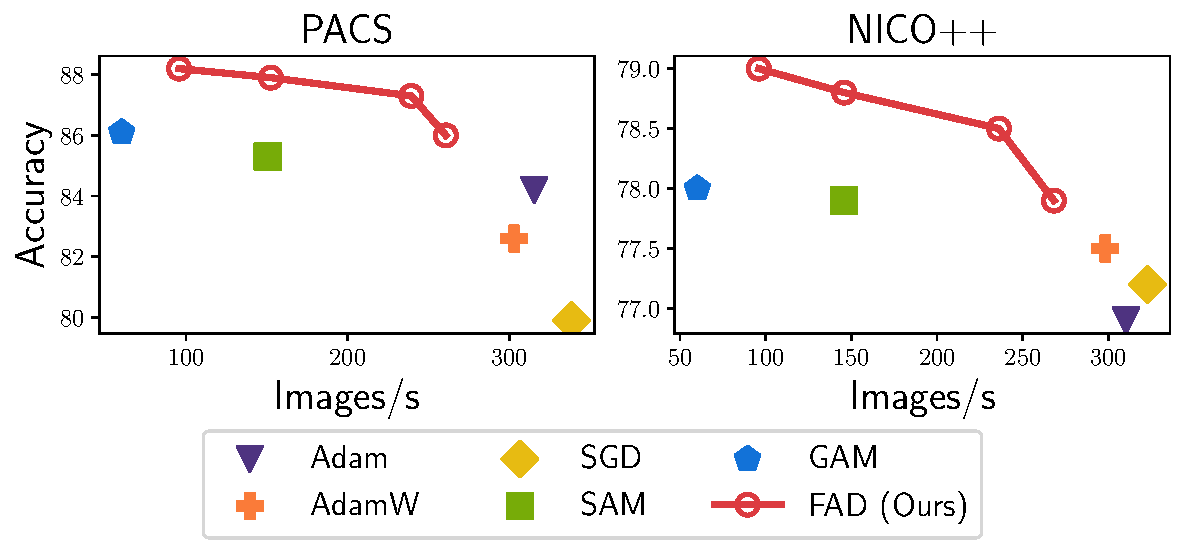
\includegraphics[width=\linewidth]{figs/efficiency.pdf}
    \caption{Comparison of computation overhead. Red points on folding lines indicate models trained with FAD for various ratios of iterations (From left to right in each figure, the proportions are 100\%, 50\%, 10\%, 5\%).}
    \label{fig:efficiency}
    \vspace{-15px}
\end{figure}

Since flatness-aware optimization methods require more computation overhead than traditional optimizers, we report the comparison of FAD with other optimizers with more training iterations. We train current optimizers on DG benchmarks for 5,000, 10,000, and 15,000 iterations. We report the performance and required average training time in Table \ref{tab:dg-cost}. Most optimizers achieve noticeable improvements in performance with more training iterations on PACS, VLCS, and OfficeHome. We show that FAD still outperforms current optimizers with fewer training iterations. For example, models trained with FAD for 5,000 iterations on PACS and NICO++ outperform those trained with other optimizers for 15,000 iterations.
This indicates the effectiveness and efficiency of FAD. 



Furthermore, as discussed in Section \ref{sect:algorithm-detail}, the FAD gradient can be efficiently calculated via first-order gradient approximation. Yet it still introduces extra computation when calculated in each iteration. Here we investigate optimizing the FAD term only for a subset of iterations in each epoch and optimize the remaining iterations simply with SGD on PACS and NICO++. We change the ratio of the subset with FAD from 5\% to 100\% and report the performance and training speed. We set the batch size to 96 (32 $\times 3$) for PACS and 128 (32 $\times 4$) for NICO++ for all the methods for a fair comparison. As shown in Figure \ref{fig:efficiency}, FAD consistently outperforms SGD, Adam, and AdamW by considerable margins and surpasses SAM and GAM with less training time when setting the ratio of FAD to 10\% and 50\%. Detailed results are in Appendix B.


\begin{table*}[th]
\centering
\caption{The performance and average training time of current optimizers and FAD when training for 5,000, 10,000, 15,000 iterations. \textit{Training Time} is the average time for finishing each dataset with the given iterations.}
\resizebox{0.735\linewidth}{!}{
\begin{tabular}{lc|c|cccc|c}
\toprule
\textbf{Optimizers} & Iterations & Training Time /s & PACS & VLCS & OfficeHome & NICO++ & \textbf{Avg.} \\
\midrule

Adam  & 5,000 & 1613.9 & 84.2 & 77.3 & 67.6 & 76.2 & 76.3 \\
Adam  & 10,000 & 3049.5 & 82.9 & 77.7 & 67.4 & 76.9 & 76.2 \\
Adam  & 15,000 & 4478.6 & 84.0 & 78.4 & 69.6 & 77.3 & 77.3 \\
% Adam \cite{} & 40,000 & & &  & & &  & &  \\
\midrule
AdamW & 5,000 & 2145.2 & 83.6 & 77.4 & 68.8 & 76.9 & 76.7 \\
AdamW  & 10,000 & 4632.8 & 83.3 & 77.1 & 66.9 & 77.5 & 76.2 \\
AdamW  & 15,000 & 6995.3 & 83.7 & 76.3 & 68.0 & 77.5 & 76.4 \\
\midrule
SGD  & 5,000  & 1864.1 & 79.9 & 78.1 & 68.5 & 76.5 & 75.8 \\
SGD  & 10,000 & 3438.9 &  81.4 & 78.1 & 68.7 & 77.2 & 76.4 \\
SGD  & 15,000 & 4992.0 & 82.6 & 78.7 & 69.6 & 77.0 & 77.0 \\
% SGD \cite{} & 40,000 & &  &  & &  &  & \\
\midrule
YOGI  & 5,000 & 1388.9 & 81.2 & 77.6 & 68.3 & 77.1 & 76.1 \\
YOGI & 10,000 & 2882.9 & 81.2  & 77.8  & 70.2 & 77.9 & 76.8 \\
YOGI  & 15,000 & 4434.2 & 83.1 & 78.1 & 67.9 & 77.5 & 76.7 \\
\midrule
SAM  & 5,000 & 3325.6 & 85.3 & 78.2 & 68.0 & 77.0 & 77.1 \\
SAM  & 10,000 & 6506.8 & 85.6 & 78.3 & 68.6 & 77.9 & 77.6 \\
SAM  & 15,000 & 9960.2 & 86.1 & 78.9 & 68.8 & 78.1 & 78.0 \\
\midrule
GAM & 5,000 & 8073.6 & 86.1 & 78.5 & 68.2 & 77.4 & 77.6 \\
GAM  & 10,000 & 16210.5 & 86.0 & 79.2 & 68.5 & 78.0 & 78.0 \\
GAM & 15,000 & 23855.1 & 86.5 & 78.6 & 69.0 & 77.8 & 78.0 \\

\midrule
FAD (Ours) & 5,000 & 5057.8 & 88.2 & 78.9 & 69.2 & 78.5 & 78.7 \\
FAD (Ours) & 10,000 & 10450.8 & 88.5 & 79.5 & 69.6 & 79.0 & 79.1 \\
FAD (Ours) & 15,000 &  16255.2 & 88.5 & 79.0 & 69.0 & 79.1 & 78.9 \\
\bottomrule
\end{tabular}}
\label{tab:dg-cost}
\end{table*}


\subsection{The Hessian spectra of selected minima}
\begin{figure*}[t]
    \centering
    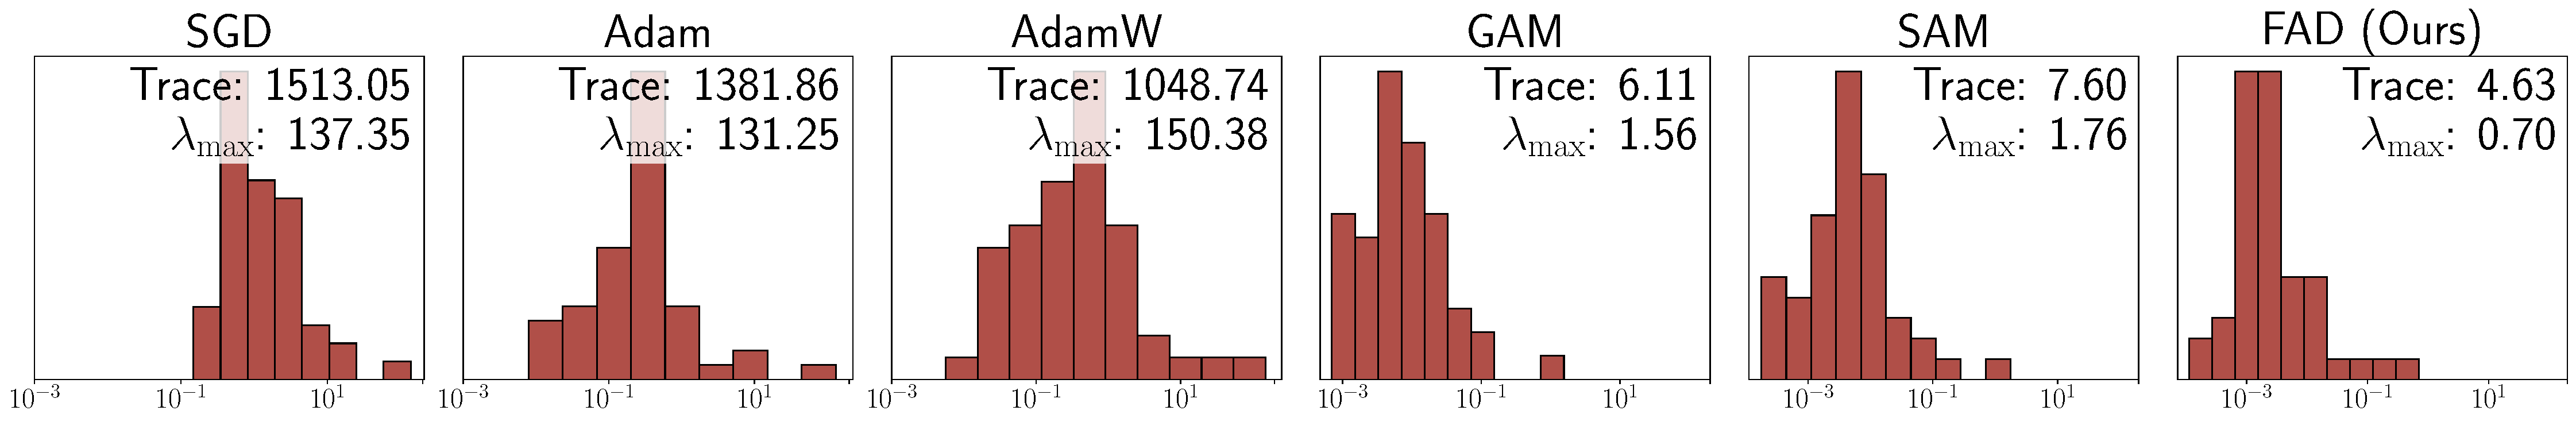
\includegraphics[width=\linewidth]{figs/eigenvalue.pdf}
    \caption{The distribution of top eigenvalues and the trace of Hessian at convergence on PACS with SGD, Adam, AdamW, GAM, SAM, and FAD. \textit{Trace} indicates Hessian trace and \textit{$\lambda_{\max}$} indicates the maximum eigenvalue of Hessian.}
    \label{fig:hessian}
\end{figure*}

Sharpness-aware optimization methods are shown to decrease the curvature of loss landscape \cite{foret2021sharpness,Zhang2023GradientNA}. We investigate how FAD affects the flatness of minima. We consider the maximum eigenvalue of Hessian, which indicates the sharpness across the most critical direction, and the Hessian trace, which measures the expected loss increase under random perturbations to the weights \cite{kaur2022maximum} as the measures of flatness. 

We show the Hessian spectra of ResNet-50 trained on art\_painting, cartoon, and photo domains of PACS for 5,000 iterations with SGD, Adam, AdamW, GAM, SAM, and FAD. Following \cite{Zhang2023GradientNA}, we adopt power iteration \cite{yao2018hessian} to compute the top eigenvalues of Hessian and Hutchinson’s method \cite{bai1996some,avron2011randomized,yao2020pyhessian} to compute the Hessian trace. We report the distribution of the top-50 Hessian eigenvalues and Hessian trace for each method at convergence in Figure~\ref{fig:hessian}. None-flatness-aware optimizers, including SGD, Adam, and AdamW show high Hessian trace and dominant eigenvalues. In contrast, flatness-aware optimizers find minima with significantly lower Hessian spectra. FAD leads to both the lowest Hessian maximum eigenvalue and trace and thus the lowest curvature compared with other optimizers. More results are shown in Appendix B.    